\label{tutorial:MutUseage} In this tutorial, we will build a 3D fully-coupled GWF-SWF model, check the build using \tecplot, run \mfus\ to generate output, then examine the results using \tecplot.

\begin{verbatim}
    ! This example builds a modflow project of the Abdul Field Experiment
    ! The SWF mesh and top of the GWF mesh are defined by a 2D Grid Builder triangular mesh
    build modflow usg
\end{verbatim}

Any input line beginning with  is considered to be a comment and will be ignored by \mut\.  Here we begin the file with two comments describing the project.

The third line activates the \mut\ 'build modflow usg' environment, which accepts further instructions required to define the project. This environment can be split into roughly 4 sections:
\begin{description}
    \item[Grid definition] Instructions for defining the GWF, SWF and CLN numerical discretizations.
    \item[Modflow parameters] Instructions for supplying Modflow parameter values (e.g. solver inputs for the SMS package, hydraulic properties for the LPF package etc.)
    \item[Stress periods, boundary conditions] These instructions are repeated once for each desired stress period and include instructions about time stepping parameters and boundary conditions that are to be applied.
    \item[Output control] Instructions defining a list of output times at which Modflow output files (e.g. heads, drawdowns, cell-by-cell flows etc.) are to be written.
\end{description}


The first group of instructions are used to build the Modflow unstructured mesh. \mut\ requires a 2D 'template'

\begin{verbatim}
    ! -----------------------------------Grid definition
    2d mesh from gb
    ./gb/grid
\end{verbatim}

\section*{Step~\ref{step:copy}: Copy an Existing \mut\ Project}

Create a new folder called e.g. \verb+My_Project+ and copy the folder \verb+MUT_Examples\6_Abdul_Prism_Cell+ into it.
Figure~\ref{fig:my_project} shows the contents of our \verb+6_Abdul_Prism_Cell+ folder.  Yours may look different depending on the root drive and folder location.
\begin{figure}[h!]
    \centering
    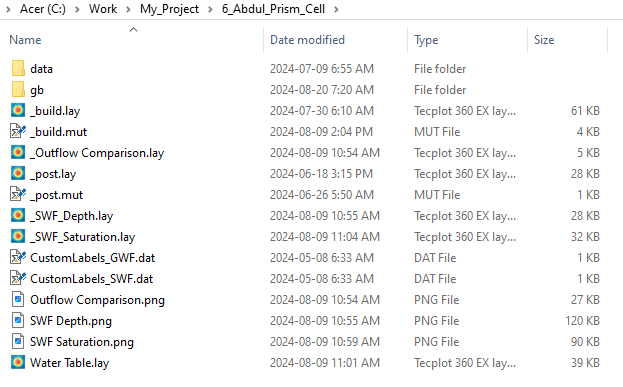
\includegraphics[width=0.8\textwidth]{abdul_folder_contents}
    \caption{The contents of the 6\_Abdul\_Prism\_Cell folder}
    \label{fig:my_project}
\end{figure}

This example contains several files you might typically find in a \mut\ Modflow project, including \mut\ input files (extension .mut), \tecplot\ layout files (extension .lay), \tecplot\ input files (extension .dat).  For now, our focus will be on the \mut\ input file \_\verb+build.mut+.

\section*{Step~\ref{step:modify}: Modify the Input File(s)}
The input file \_\verb+build.mut+ is set up to build a Modflow project.  If you open the file in a text editor you will see that it consists of a sequence of comments (lines beginning with an exclamation mark \verb+!+), \mut\ instructions and data (numbers or alphanumeric strings).  Details of the input file contents are described in detail in Section~\ref{InputFileDetails}.  For now, we will only make a minor change to the input file before moving on to the next step, which is to add a new comment line of your choice at the start of the file.

\section*{Step~\ref{step:mut1}: Execute \mut\ to Build the Project}


Assuming you have followed the set-up instructions in Section~\ref{Install}, you can execute \mut\ with the input file \_\verb+build.mut+ by typing:
\begin{verbatim}
    mut _build
\end{verbatim}


\section*{Step~\ref{step:Tecplot1}: Run \tecplot\ to Examine the Built Project}
You can run \tecplot\ and load the \tecplot\ layout file \_\verb+build.lay+ by typing:
\begin{verbatim}
    tec360 _build.lay
\end{verbatim}
Note the following:
\begin{itemize}
    \item A \tecplot\ window should open: \\ \\
        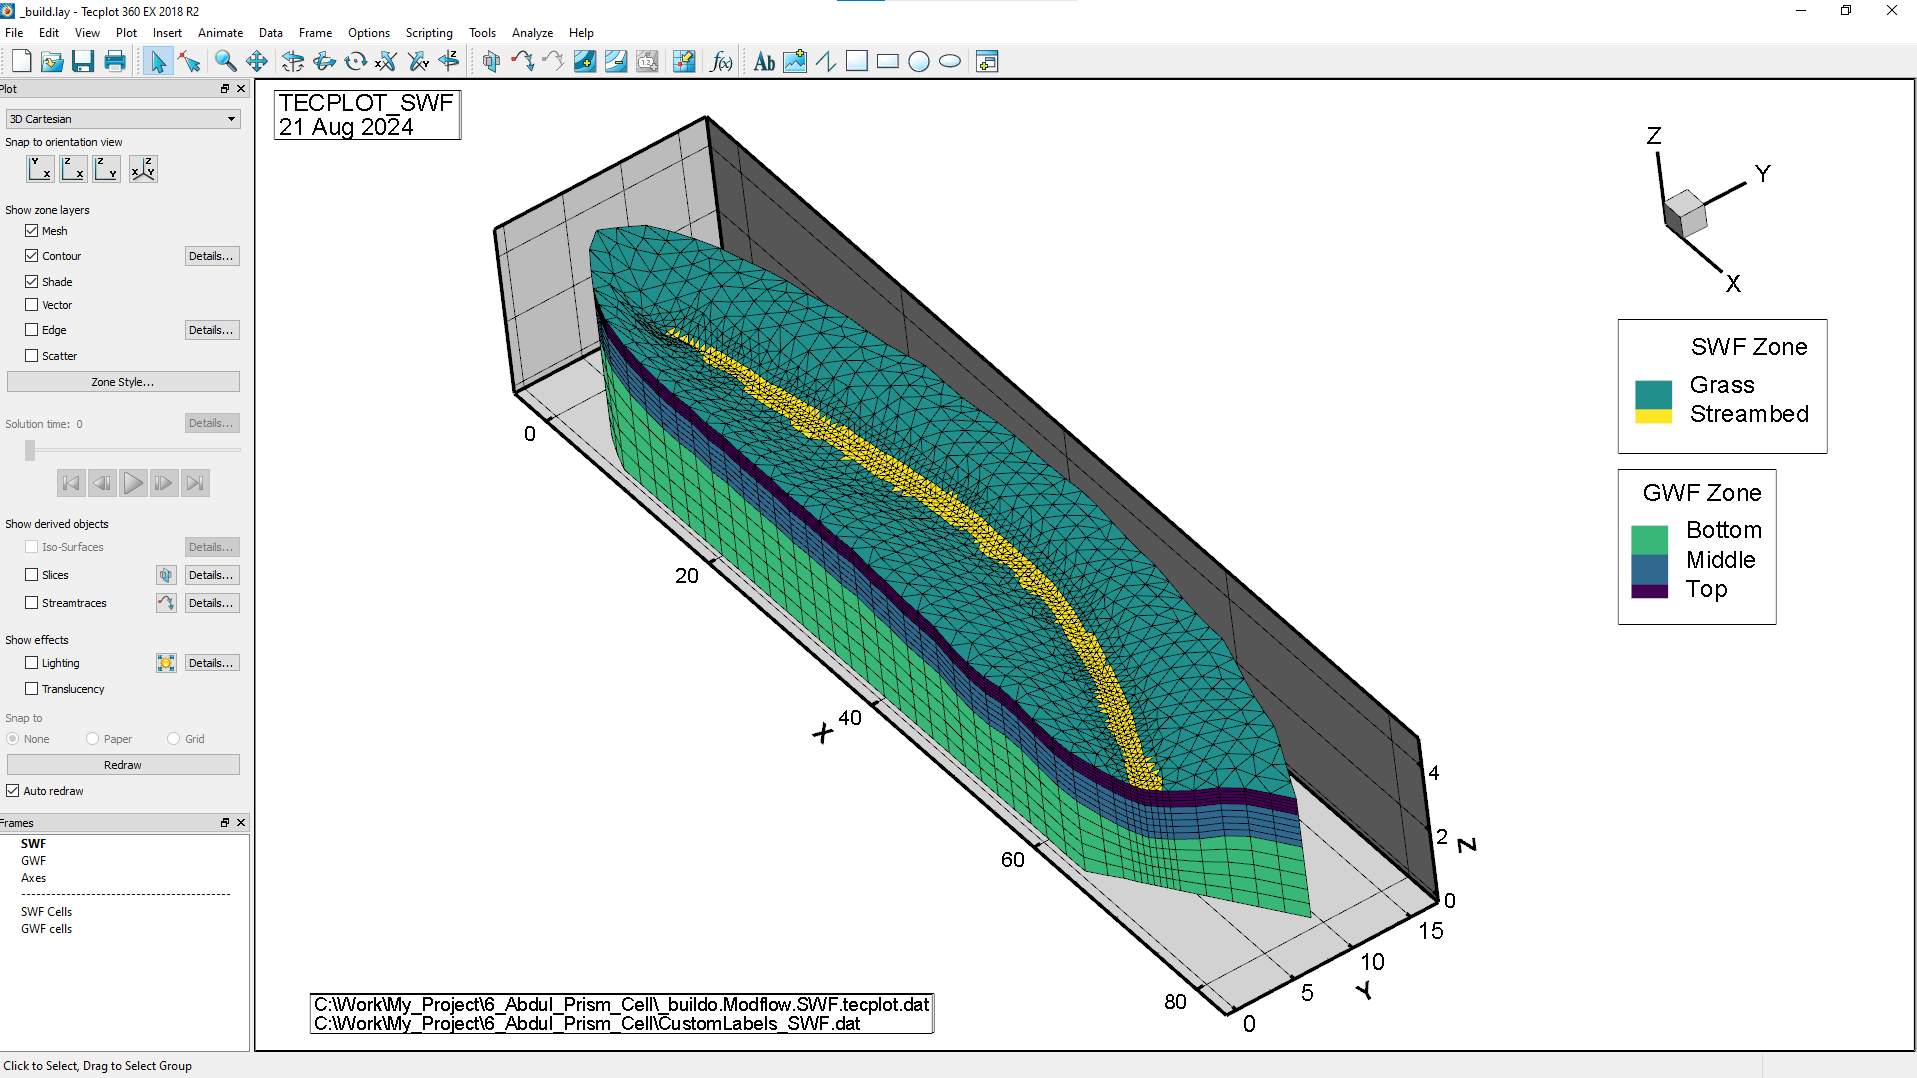
\includegraphics[width=0.8\textwidth]{TecplotBuild} \\ \\
    This \tecplot\ layout file has been constructed with multiple frames (see lower left 'Frames' window) showing details about the SWF and GWF model domains. This default view shows the distribution of the various materials defined in the model, such as the SWF domain materials called 'Grass' and 'Streambed'.  Detailed information about manipulating the data in \tecplot\ to produce the desired plots is discussed in Section~\ref{Tecplot}.
    \item \tecplot\ data can be probed using the probe tool 
\includegraphics{ProbeToolButton} .  Here we see the results of probing a location in the SWF domain: \\
        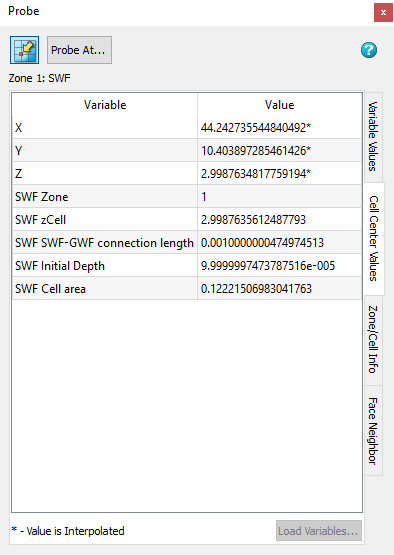
\includegraphics[width=0.4\textwidth]{SWFprobe} \\
        SWF results were returned because the SWF frame is at the front of the frame stack.
    \item In order to probe the GWF domain we have to move it to the front of the stack: \\
            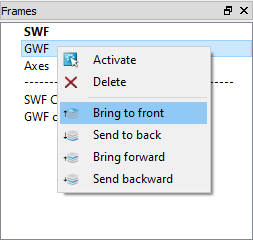
\includegraphics[width=0.4\textwidth]{BringToFront} \\
          Here we see the results of probing a location in the GWF domain: \\
            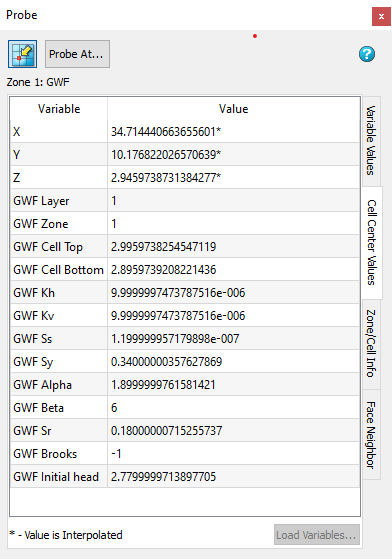
\includegraphics[width=0.4\textwidth]{GWFprobe} \\

\end{itemize}



\section*{Step~\ref{step:modflow}: Run Modflow to Generate Output}
\section*{Step~\ref{step:mut2}: Run \mut\ to Post-Process the Modflow Output}
\section*{Step~\ref{step:Tecplot2}: Run \tecplot\ to Visualize the Modflow Output}

